\section{Introduction}

\begin{frame}{Adversarial Examples}

    \begin{alertblock}{Definition}
        Adversarial examples are carefully crafted input data designed to cause an AI system to produce incorrect or biased predictions (Szegedy et al., 2014).
    \end{alertblock}
    \begin{center}
        \begin{figure}
            \includegraphics[width=0.70\linewidth]{img/AdvExample.png}
            \\ {\tiny Source: Szegedy et al. Explaining and harnessing adversarial examples}
        \end{figure}
    \end{center}

\end{frame}

\begin{frame}{Why do we care ?}

    \begin{itemize}
        \item Adversarial examples pose a significant security risks in safety-critical domains (e.g., healthcare, autonomous transportation, etc.)
        \begin{itemize}
            \item Compromised security systems;
            \item Data breaches and unauthorized access;
            \item Financial losses and fraud;
            \item \dots
        \end{itemize}
    \end{itemize}

\end{frame}

\begin{frame}[fragile]{$k$-NN}
    \begin{itemize}
        \item A \emph{non-parametric} supervised machine learning method;
        \item Suitable for both classification and regression tasks;
        \item Leverages data similarity to compute the prediction;
        \item Relies on distance metrics like Euclidean\\Manhattan or the general Minkowski distance;
    \end{itemize}

\end{frame}

\begin{frame}[fragile]{$3$-NN}
    \begin{figure}[H]
        \centering
        \usetikzlibrary{arrows.meta, intersections}
        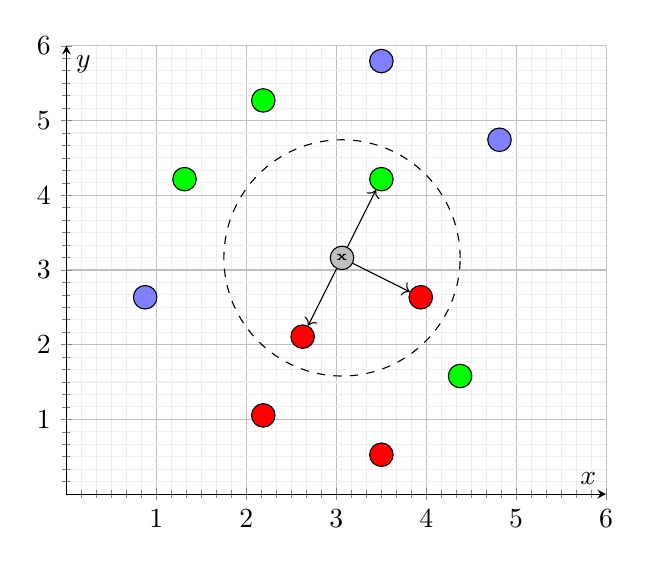
\begin{tikzpicture}[
            dot/.style = {circle, draw, fill=#1, inner sep=3pt, node contents={}}
        ]
            \begin{axis}[
                xmin = 0, xmax = 6,
                ymin = 0, ymax = 6,
                xtick distance = 1,
                ytick distance = 1,
                grid = both,
                minor tick num = 5,
                major grid style = {lightgray},
                minor grid style = {lightgray!25},
                axis x line=center,
                axis y line=center,
                xlabel = {$x$},
                ylabel = {$y$},
                xlabel style={above left},
                ylabel style={below right}
            ]
            \node (x) at (3.5cm,3cm) [dot=gray!50];
            \node (l_x) at (3.5cm,3cm) {\textbf{\tiny x}};
			\node (c) at (3.5cm,3cm) [circle, draw, dashed, inner sep=0pt, minimum size=3cm, name path=C] {};
			\node (p1) at (2.5cm,5cm) [dot=green];
			\node (p2) at (4cm,4cm) [dot=green];
			\node (p3) at (5cm,1.5cm) [dot=green];
			\node (p4) at (1.5cm,4cm) [dot=green];
			\node (p5) at (1cm,2.5cm) [dot=blue!50];
			\node (p6) at (4cm,5.5cm) [dot=blue!50];
			\node (p6) at (5.5cm,4.5cm) [dot=blue!50];
			\node (p7) at (4cm,0.5cm) [dot=red];
			\node (p8) at (4.5cm,2.5cm) [dot=red];
			\node (p9) at (3cm,2cm) [dot=red];
			\node (p10) at (2.5cm,1cm) [dot=red];
			\draw [->] (x) -- (p2);
			\draw [->] (x) -- (p8);
			\draw [->] (x) -- (p9);
            \end{axis}
        \end{tikzpicture}
    \end{figure}
    \begin{center}
        \tiny 3NN over a dataset with 3 classes, which shows how a new  point is classified
    \end{center}
\end{frame}

\begin{frame}[fragile]{$3$-NN}
    \begin{figure}[H]
        \centering
        \usetikzlibrary{arrows.meta, intersections}
        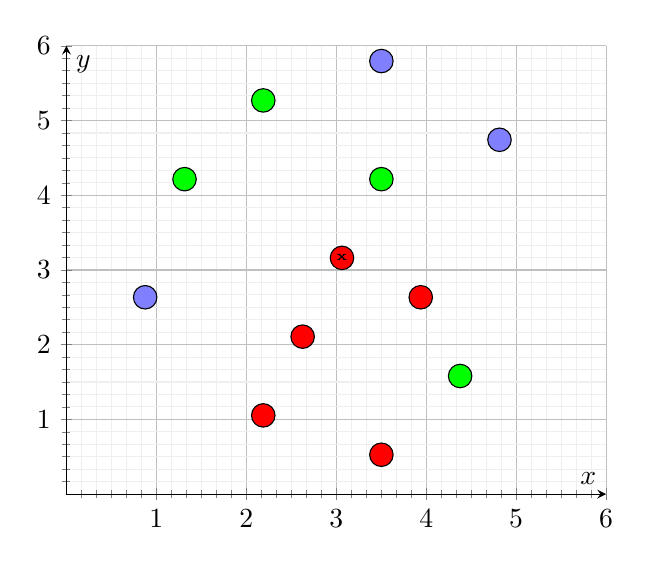
\begin{tikzpicture}[
            dot/.style = {circle, draw, fill=#1, inner sep=3pt, node contents={}}
        ]
            \begin{axis}[
                xmin = 0, xmax = 6,
                ymin = 0, ymax = 6,
                xtick distance = 1,
                ytick distance = 1,
                grid = both,
                minor tick num = 5,
                major grid style = {lightgray},
                minor grid style = {lightgray!25},
                axis x line=center,
                axis y line=center,
                xlabel = {$x$},
                ylabel = {$y$},
                xlabel style={above left},
                ylabel style={below right}
            ]
            \node (m) at (3.5cm,3cm) [dot=red];
            \node (l_x) at (3.5cm,3cm) {\textbf{\tiny x}};
    		\node (p1) at (2.5cm,5cm) [dot=green];
			\node (p2) at (4cm,4cm) [dot=green];
			\node (p3) at (5cm,1.5cm) [dot=green];
			\node (p4) at (1.5cm,4cm) [dot=green];
			\node (p5) at (1cm,2.5cm) [dot=blue!50];
			\node (p6) at (4cm,5.5cm) [dot=blue!50];
			\node (p6) at (5.5cm,4.5cm) [dot=blue!50];
			\node (p7) at (4cm,0.5cm) [dot=red];
			\node (p8) at (4.5cm,2.5cm) [dot=red];
			\node (p9) at (3cm,2cm) [dot=red];
			\node (p10) at (2.5cm,1cm) [dot=red];
            \end{axis}
        \end{tikzpicture}
    \end{figure}
    \begin{center}
        \tiny 3NN over a dataset with 3 classes, which shows how a new  point is classified
    \end{center}
\end{frame}

\begin{frame}{Goal}

    \begin{itemize}
        \item Exact robustness certification of the $k$-Nearest Neighbors Classifier;
        \item Focus on \emph{completeness};
        \item Consider only the Euclidean distance as similarity metric.
    \end{itemize}
\end{frame}